\documentclass[11pt]{amsart}
\usepackage[a4paper,margin=1in]{geometry}
\usepackage{amsmath,amssymb,amsthm}
\usepackage{tikz}
\usepackage[hidelinks]{hyperref}

\newtheorem{theorem}{Theorem}[section]
\newtheorem{lemma}[theorem]{Lemma}
\newtheorem{proposition}[theorem]{Proposition}
\newtheorem{corollary}[theorem]{Corollary}
\theoremstyle{definition}
\newtheorem{definition}[theorem]{Definition}
\newtheorem{rem}[theorem]{Remark}
\newtheorem{question}[theorem]{Question}

\title[Common quartets of several phylogenetic trees]{Common quartets of several phylogenetic trees:\\
$h(3)=14$ and exponential bounds for $h(k)$}
\author{Vamshi Jandhyala}
\address{London, United Kingdom}
\email{vamshi.jandhyala@gmail.com}
\date{Preprint v1, 20 October 2026}
\subjclass[2020]{05C05, 05D10, 92D15}
\keywords{phylogenetic tree, quartet, caterpillar, agreement subtree, SAT}

\begin{document}

\begin{abstract}
Let $h(k)$ be the least $n$ such that any $k$ unrooted binary phylogenetic trees on the same $n$ leaves display a
common quartet. Snir and Yuster asked for its value; it was known that $h(2)=6$ and $11\le h(3)\le 14$, and the
best published upper bound for general $k$ was a four-times iterated exponential. We show $h(3)=14$ and
$h(k)\le 2\cdot 3^{k-1}+1$ for every $k\ge 2$. The upper bound applies to trees the iteration of Spencer's
two-bipartition lemma that Asplund, Do, Hamm, Sz\'ekely, Taylor and Wang used for $k$-planar crossing numbers. Snir
and Yuster stated that caterpillars give $h(k)\ge 2^k+2$ and omitted the construction; we give an explicit family of
$k$ caterpillars on $2^k+1$ leaves, built by reflecting leaf orders according to binary digits, with a proof. The
value $h(3)=14$ needs three trees on $13$ leaves with no common quartet; we give one of the form $T$, $3T$, $9T$ on
$\mathbb{Z}_{13}$, and confirm the matching upper bound by an exhaustive search with checked proofs. Up to the
symmetries of this form there are exactly six such examples. We also find
four trees on $21$ leaves with no common quartet, so $h(4)\ge 22$. The general bounds and the $13$-leaf example are
checked in Lean.
\end{abstract}

\maketitle

\section{Introduction}

Given $k$ evolutionary trees on the same species, how many species force them all to agree on the shape of some
four-species subtree? This note answers the question for three trees and narrows it for every $k$.

A phylogenetic tree on a leaf set $X$ is an unrooted tree whose internal vertices have degree three and whose leaves
are labelled bijectively by $X$. Four leaves $a,b,c,d$ induce one of three binary trees, written $ab|cd$, $ac|bd$ or
$ad|bc$; this is the \emph{quartet} the tree displays on $\{a,b,c,d\}$, and $ab|cd$ means that some edge has $a,b$
on one side and $c,d$ on the other. A tree is determined by its quartets \cite{CS,BD}. Comparing trees through
their quartets is standard in phylogenetics, and a basic extremal question is how different several trees on the
same species can be. Two random trees agree, in expectation, on a third of their quartets, yet two trees can avoid
agreeing altogether when there are few leaves. Figure~\ref{fig:five} shows two trees on five leaves with no quartet
in common. On six or more leaves this is impossible: any two trees share a quartet \cite{BD}.

\begin{figure}[ht]
\centering
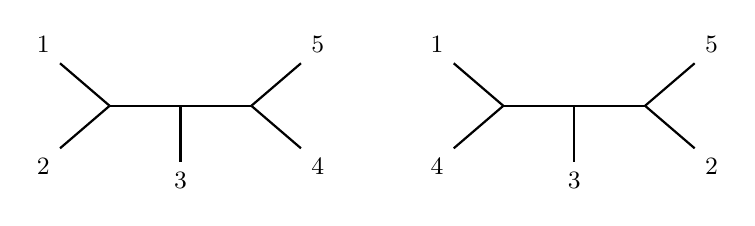
\begin{tikzpicture}[x=0.9cm,y=0.9cm,every node/.style={font=\small}]
\foreach \ox/\a/\b/\c/\d/\e in {0/1/2/3/4/5, 5/1/4/3/2/5} {
  \begin{scope}[xshift=\ox cm]
  \draw[thick] (1,0) -- (3,0);
  \draw[thick] (1,0) -- (0.3,0.6) node[above left] {$\a$};
  \draw[thick] (1,0) -- (0.3,-0.6) node[below left] {$\b$};
  \draw[thick] (2,0) -- (2,-0.8) node[below] {$\c$};
  \draw[thick] (3,0) -- (3.7,-0.6) node[below right] {$\d$};
  \draw[thick] (3,0) -- (3.7,0.6) node[above right] {$\e$};
  \end{scope}
}
\end{tikzpicture}
\caption{Two trees on five leaves with no common quartet. Each quartet is the four leaves left after deleting one.
Deleting $5$ gives $12|34$ in the left tree and $14|23$ in the right; deleting $1$ gives $23|45$ and $25|34$; the
other three quartets differ in the same way. The right tree reverses the middle three leaves of the left one, the
move that drives the construction in Section~\ref{sec:lower}.}
\label{fig:five}
\end{figure}

Snir and Yuster \cite[\S5]{SY} asked for the least $n$ such that any $k$ phylogenetic trees on $[n]$ display a
common quartet, and denoted it $h(k)$. The result of Bandelt and Dress gives $h(2)=6$. For caterpillars (trees in
which every internal vertex lies on one path) Snir and Yuster stated that the analogous number is $h^*(k)=2^k+2$,
proving the upper bound and giving the construction for the lower bound only for $k=3$. Three trees on ten leaves
with no common quartet \cite[Figure~4]{SY} and their separation theorem \cite[Theorem~1.3]{SY} give
$11\le h(3)\le 14$. Currie, Czabarka, Fischer, Simmons, Sz\'ekely and Wicke \cite{CCFSSW} proved
$8^{1/4}3^{k/4}\le h(k)\le \mathrm{tw}_3\bigl(6(k-1)2^k+O(\log k)\bigr)$, a four-times iterated exponential, the
upper bound through hypergraph Ramsey numbers and agreement subtrees.

\begin{theorem}\label{thm:h3}
$h(3)=14$.
\end{theorem}

\begin{theorem}\label{thm:hk}
For every $k\ge 2$, \quad $2^k+2\le h(k)\le 2\cdot 3^{k-1}+1$.
\end{theorem}

\begin{theorem}\label{thm:h4}
$22\le h(4)\le 55$, and $h(4)\le 41$ given the error-free form of \cite[Theorem~1.3]{SY}.
\end{theorem}

The lower bound in Theorem~\ref{thm:hk} is $h(k)\ge h^*(k)$, since caterpillars are trees, and the value
$h^*(k)=2^k+2$ is Snir and Yuster's; Section~\ref{sec:lower} supplies the construction they omitted, an explicit
family of $k$ caterpillars on $2^k+1$ leaves with no common quartet, with a short proof. The upper bound
(Section~\ref{sec:upper}) iterates a lemma of Spencer, as Asplund et al.\ \cite{ADHSTW} did for $k$-planar crossing
numbers: each further tree costs a factor of three in the size of two sets that every tree separates, and two such
sets of size two already give a common quartet. Starting the iteration from Snir and Yuster's three-tree theorem
gives $h(k)\le\lfloor 3^k/2\rfloor+1$ for $k\ge3$, which is $14$ for $k=3$ and $41$ for $k=4$. The proof of that
theorem without its error term is given in \cite{SY} in outline, so we state the bounds that rest on it separately.

For three trees the lower bound $2^3+2=10$ is far from the truth. Section~\ref{sec:h3} gives three trees on $13$
leaves with no common quartet, in a symmetric form: a single tree $T$ on $\mathbb{Z}_{13}$ together with its images
under $x\mapsto 3x$ and $x\mapsto 9x$. The upper bound $h(3)\le14$ is Snir and Yuster's, whose proof of the
error-free form of their separation theorem is a sketch; we confirm it independently by an exhaustive SAT search
over the $135$ shapes of the first tree, each unsatisfiable instance carrying a checked proof.

The gap between $2^k$ and $3^k$ is the main question left open (Section~\ref{sec:open}). The data $h(2)=6$,
$h(3)=14$, $h(4)\ge22$ beat the caterpillar values $6,10,18$ from $k=3$ on.

\section{Separated sets}\label{sec:prelim}

For a tree $T$ on $X$ and disjoint $A,B\subseteq X$, say $T$ \emph{separates} $A$ and $B$ if some edge of $T$ has
$A$ on one side and $B$ on the other. Then $T$ displays $ab|cd$ exactly when it separates $\{a,b\}$ and $\{c,d\}$, and
if $T$ separates $A$ and $B$ it separates any subsets of them. For $U\subseteq X$ the restriction $T|U$ is the
phylogenetic tree obtained from the subtree spanning $U$ by suppressing vertices of degree two. An edge of $T|U$
comes from a path of $T$, and deleting any edge of that path splits $U$ the same way; so a split $C|U\setminus C$ of
$T|U$ means that $T$ separates $C$ and $U\setminus C$.

\begin{lemma}[folklore; see {\cite[Lemma~3.1]{SY12}}]\label{lem:third}
Every phylogenetic tree on $N\ge2$ leaves has an edge whose removal leaves at least $N/3$ leaves on each side.
\end{lemma}

\begin{proof}
Choose an edge $e$ whose larger side $S$ has as few leaves as possible, and suppose $|S|>2N/3$. Then $|S|\ge2$, so
the end of $e$ in $S$ is an internal vertex, and its two other edges split $S$ into $S_1\sqcup S_2$ with, say,
$|S_1|\ge|S|/2>N/3$. The edge leading to $S_1$ has sides of sizes $|S_1|<|S|$ and $N-|S_1|<2N/3<|S|$, contradicting
the choice of $e$. So $|S|\le2N/3$ and the other side has at least $N/3$ leaves.
\end{proof}

\begin{lemma}[Spencer {\cite{Spencer}}; see {\cite[Lemma~6]{ADHSTW}} and {\cite[Theorem~3]{CCFSSW}}]\label{lem:cell}
Let $U=X_1\sqcup X_2=C_1\sqcup C_2$ be two bipartitions with every part of size at least $|U|/3$. Then either
$X_1\cap C_1$ and $X_2\cap C_2$, or $X_1\cap C_2$ and $X_2\cap C_1$, both have size at least $|U|/6$.
\end{lemma}

\begin{proof}
Call a cell small if it has fewer than $|U|/6$ elements. If the lemma fails, each of the two pairs of opposite cells
contains a small cell. Any cell of the first pair shares a row or a column with any cell of the second, so two small
cells lie in one part, which then has fewer than $|U|/3$ elements.
\end{proof}

\begin{figure}[ht]
\centering
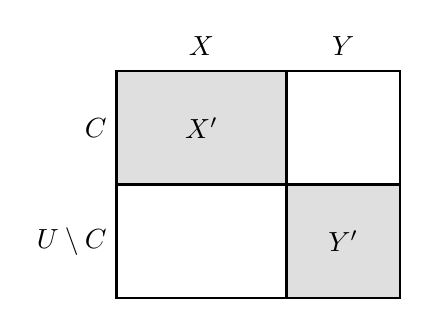
\begin{tikzpicture}[scale=0.9]
\fill[gray!25] (0,1.6) rectangle (2.4,3.2);
\fill[gray!25] (2.4,0) rectangle (4,1.6);
\draw[thick] (0,0) rectangle (4,3.2);
\draw[thick] (2.4,0) -- (2.4,3.2);
\draw[thick] (0,1.6) -- (4,1.6);
\node at (1.2,3.55) {$X$};
\node at (3.2,3.55) {$Y$};
\node[left] at (0,2.4) {$C$};
\node[left] at (0,0.8) {$U\setminus C$};
\node at (1.2,2.4) {$X'$};
\node at (3.2,0.8) {$Y'$};
\end{tikzpicture}
\caption{One step of the iteration. The earlier trees separate $X$ and $Y$; the new tree, restricted to
$U=X\cup Y$, splits $U$ into $C$ and $U\setminus C$. Lemma~\ref{lem:cell} finds opposite cells $X'$, $Y'$ of
at least a sixth of $U$, and every tree separates them.}
\label{fig:cell}
\end{figure}

\section{The upper bound}\label{sec:upper}

The following proposition is the iteration in the proof of Theorem~2 of Asplund et al.\ \cite{ADHSTW}, where the
bipartitions are $1/3$--$2/3$ bisections of graphs; here they come from tree edges through Lemma~\ref{lem:third}. We
include the short proof to keep the note self-contained.

\begin{proposition}\label{prop:upper}
Let $k\ge2$ and let $T_1,\dots,T_k$ be phylogenetic trees on a set of $n$ leaves. There are disjoint sets $X,Y$
separated by every $T_i$ with $2\cdot3^{k-1}|X|\ge n$ and $2\cdot3^{k-1}|Y|\ge n$.
\end{proposition}

\begin{proof}
Induction on $k$. For $k=2$, Lemma~\ref{lem:third} gives a split $X_1|X_2$ of the leaf set displayed by $T_1$ and a
split $C_1|C_2$ displayed by $T_2$, all four parts of size at least $n/3$; Lemma~\ref{lem:cell} gives opposite cells
of size at least $n/6$, separated by both trees.

Suppose $X,Y$ work for $T_1,\dots,T_{k}$. Shrink them to subsets $X_0,Y_0$ of a common size $m=\min(|X|,|Y|)$ and
let $U=X_0\cup Y_0$, so $|U|=2m$. By Lemma~\ref{lem:third} applied to $T_{k+1}|U$, the tree $T_{k+1}$ separates
some $C$ and $U\setminus C$ with $|C|,|U\setminus C|\ge 2m/3=|U|/3$. Both parts of $X_0\sqcup Y_0$ have size
$m\ge|U|/3$, so Lemma~\ref{lem:cell} gives $X'\subseteq X_0$ and $Y'\subseteq Y_0$, one inside $C$ and the other
inside $U\setminus C$, each of size at least $|U|/6=m/3$ (Figure~\ref{fig:cell}). Then $T_{k+1}$ separates $X'$ and
$Y'$, the earlier trees do because $X'\subseteq X$ and $Y'\subseteq Y$, and
$2\cdot3^{k}|X'|\ge 2\cdot3^{k-1}m\ge n$.
\end{proof}

\begin{proof}[Proof of the upper bounds in Theorems~\ref{thm:hk} and \ref{thm:h4}]
If $n\ge2\cdot3^{k-1}+1$ then $|X|,|Y|>1$ in Proposition~\ref{prop:upper}. Choose $a,b\in X$ and $c,d\in Y$: every
tree separates $\{a,b\}$ and $\{c,d\}$, so every tree displays $ab|cd$. For $k=4$ this gives $55$. For $k\ge3$,
starting the induction at $k=3$ from the error-free form of \cite[Theorem~1.3]{SY}, which gives separated sets with
$27|X|,27|Y|\ge 2n$, yields $\tfrac12 3^{k}|X|\ge n$ and hence $h(k)\le\lfloor 3^k/2\rfloor+1$; for $k=4$ this is
$41$.
\end{proof}

\section{Caterpillars on $2^k+1$ leaves with no common quartet}\label{sec:lower}

A caterpillar is determined, up to reversal, by the order in which its leaves meet the spine, and the caterpillar
with order $x_1,\dots,x_n$ displays $x_px_q|x_rx_s$ whenever $p<q<r<s$. We describe a caterpillar by a
\emph{position map}: a bijection from the leaves to $\mathbb{Z}$ whose order is the leaf order.

\begin{definition}\label{def:Fk}
Let $k\ge1$ and $h=2^{k-1}$. The leaves are the integers $-h,\dots,h$. The caterpillar $\pi_0$ has the identity
position map. For $0\le b\le k-2$, the caterpillar $\pi_{b+1}$ puts leaf $x$ at position $-x$ if $x\ne0$ and the
binary digit of $|x|-1$ in place $b$ is $0$, and at position $x$ otherwise. Let $F_k=\{\pi_0,\dots,\pi_{k-1}\}$.
\end{definition}

Each $\pi_j$ swaps some pairs $\{-d,d\}$ and fixes the rest, so it is a bijection of $\{-h,\dots,h\}$ fixing $0$.
For $k=3$ the three leaf orders are
\[
\begin{array}{rrrrrrrrrr}
\pi_0:& -4&-3&-2&-1&0&1&2&3&4\\
\pi_1:& -4&3&-2&1&0&-1&2&-3&4\\
\pi_2:& -4&-3&2&1&0&-1&-2&3&4
\end{array}
\]
and any four of the nine leaves are split differently by at least two of them. Relabelling $x\mapsto x+5$ turns
these into the three orders $123456789$, $127654389$, $183654729$ of Snir and Yuster's example \cite[\S5]{SY} (the
first is printed there as $12345679$), so $F_k$ extends their construction to every $k$.

\begin{theorem}\label{thm:cat}
No quartet is displayed by all the caterpillars of $F_k$.
\end{theorem}

\begin{proof}
Induction on $k$; for $k=1$ there are three leaves. Assume the result for $F_k$, with $h=2^{k-1}$, and consider
$F_{k+1}$ on $[-2h,2h]$. Write $I=[-h,h]$ for the inner leaves and $L=[-2h,-h-1]$, $R=[h+1,2h]$. Let
$\pi_{\mathrm{top}}=\pi_{k}$ be the caterpillar of the highest digit. Four facts follow from the definition
(Figure~\ref{fig:double}).
\begin{enumerate}
\item On $I$, the caterpillars $\pi_0,\dots,\pi_{k-1}$ of $F_{k+1}$ have the same position maps as those of $F_k$.
\item For an outer leaf $x$ let $\psi(x)=x-h$ if $x>0$ and $x+h$ if $x<0$, so $\psi$ maps $L\cup R$ onto
$I\setminus\{0\}$. The digits of $|x|-1$ and $|\psi(x)|-1$ agree in places below $k-1$, so for $j<k$ the position
of $x$ in $\pi_j$ is $g(\text{position of }\psi(x)\text{ in }\pi_j)$, where $g(y)=y+h$ for $y>0$ and $y-h$ for
$y<0$; and $g$ is increasing.
\item $\pi_{\mathrm{top}}$ reverses $I$ and fixes every outer leaf.
\item In every caterpillar, inner leaves sit at positions in $[-h,h]$ and outer leaves at positions outside it.
\end{enumerate}
Suppose all of $F_{k+1}$ display $ab|cd$, and let $Q=\{a,b,c,d\}$.

\emph{At most one leaf of $Q$ is inner.} Map each outer leaf by $\psi$ and the inner leaf, if any, to $0$. By (2)
and (4) the relative order of the four positions in $\pi_j$ ($j<k$) is the relative order of the images in the
$\pi_j$ of $F_k$, so $F_k$ displays a common quartet, contrary to induction.

\emph{All four leaves are inner.} By (1) and induction.

\emph{Three inner leaves and one outer leaf $y$.} In $\pi_0$ and $\pi_{\mathrm{top}}$ the leaf $y$ is at the same
end, and the inner three are in opposite orders; so $y$ is paired with different inner leaves.

\emph{Two inner leaves $u<v$ and two outer leaves $y,z$.} If $y$ and $z$ lie on opposite sides in $\pi_0$, then
$\pi_0$ pairs each with the nearer of $u,v$, and $\pi_{\mathrm{top}}$, which swaps $u$ and $v$, pairs them the other
way. If they lie on the same side then $|y|\ne|z|$, so $|y|-h-1$ and $|z|-h-1$, two different numbers below
$h=2^{k-1}$, differ in some place $b<k-1$. Then $\pi_{b+1}$ moves exactly one of $y,z$ to the other side, and it pairs
each of them with an inner leaf, while $\pi_0$ displays $yz|uv$.
\end{proof}

\begin{figure}[ht]
\centering
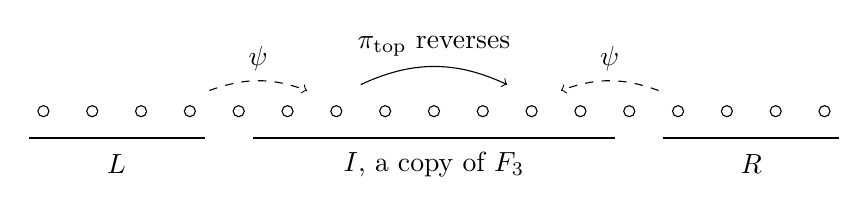
\begin{tikzpicture}[x=0.62cm,y=0.75cm]
\foreach \x in {-8,...,8} { \draw (\x,0) circle (2pt); }
\draw[thick] (-8.3,-0.45) -- (-4.7,-0.45);
\draw[thick] (-3.7,-0.45) -- (3.7,-0.45);
\draw[thick] (4.7,-0.45) -- (8.3,-0.45);
\node at (-6.5,-0.9) {$L$};
\node at (0,-0.9) {$I$, a copy of $F_3$};
\node at (6.5,-0.9) {$R$};
\draw[->] (-1.5,0.45) to[bend left=25] node[above]{$\pi_{\mathrm{top}}$ reverses} (1.5,0.45);
\draw[->,dashed] (-4.6,0.35) to[bend left=20] node[above]{$\psi$} (-2.6,0.35);
\draw[->,dashed] (4.6,0.35) to[bend right=20] node[above]{$\psi$} (2.6,0.35);
\end{tikzpicture}
\caption{The doubling step from $F_3$ to $F_4$. The inner nine leaves carry $F_3$; the outer eight form a copy of
$F_3$ without its centre, folded in by $\psi$; the new caterpillar reverses the inner block and fixes the rest.}
\label{fig:double}
\end{figure}

\begin{corollary}
$h(k)\ge h^*(k)=2^k+2$ for every $k\ge1$.
\end{corollary}

The upper bound $h^*(k)\le 2^k+2$ is Snir and Yuster's halving argument \cite[\S5]{SY}. The choice of digit place
is not essential: using the digits of $|x|$ instead of $|x|-1$ gives another family with the same property for
$k\le4$, which we checked by computer.

\section{Three trees}\label{sec:h3}

\begin{proposition}\label{prop:13}
Let $T$ be the phylogenetic tree on $\mathbb{Z}_{13}$ with Newick form
\[
\bigl(0,\,1,\,(((8,11),((5,(4,6)),((3,9),(12,(7,10))))),\,2)\bigr),
\]
and let $3T$ and $9T$ be its images under $x\mapsto3x$ and $x\mapsto9x$. No quartet is displayed by all of $T$,
$3T$ and $9T$.
\end{proposition}

The proof is a finite check of the $\binom{13}{4}=715$ quartets, done in Lean by \texttt{decide} and by an
independent script (Section~\ref{sec:verify}). The example was found by a SAT search in which the second and third
trees were forced to be the images of the first under a permutation of order three; without the symmetry
constraint the search also finds examples at once. Section~\ref{sec:z13} describes every example of this symmetric
form; we do not know a conceptual reason why they work.

\begin{proof}[Proof of Theorem~\ref{thm:h3}]
Proposition~\ref{prop:13} gives $h(3)\ge14$, and Theorem~1.3 of \cite{SY} gives $h(3)\le14$, since
$\lceil 2\cdot14/27\rceil=2$. Because the error-free form of that theorem is proved there in outline, we confirmed
$h(3)\le14$ directly. A choice of one split for every $4$-subset is the quartet set of a phylogenetic tree if and
only if its restriction to every $5$-subset is \cite{CS} (see \cite{HMSW} for this formulation). This gives a
propositional formula whose models are triples of trees on $14$ leaves with no common quartet. A permutation of the
leaves applied to all three trees preserves the property of having no common quartet, so we may take the first tree
to be a fixed representative of its shape; there are $135$ shapes of phylogenetic trees with $14$ leaves. All $135$
formulas are unsatisfiable. Each was solved by CaDiCaL~2.1.3 \cite{cadical}, which wrote an LRAT proof of
unsatisfiability, and each proof was accepted by the independent checker \texttt{lrat-check} \cite{lrat}. The
proofs total $32.6$~GB and were deleted after checking; the archive contains the scripts that regenerate and check
them (about $5{,}500$~s of solver time) and the logs of the run.
\end{proof}

\begin{proof}[Proof of the lower bound in Theorem~\ref{thm:h4}]
Let $\sigma$ be the permutation of $\{0,\dots,20\}$ that fixes $0$ and is the product of the $4$-cycles
\[
(1\,2\,3\,4)\,(5\,6\,7\,8)\,(9\,10\,11\,12)\,(13\,14\,15\,16)\,(17\,18\,19\,20),
\]
and let $T$ be the tree
\[
\begin{gathered}
(0,\,16,\,((17,10),(1,((((((6,14),11),5),((3,15),8)),\\
((4,13),(18,((20,7),19)))),(9,(2,12)))))).
\end{gathered}
\]
Then $T$, $\sigma T$, $\sigma^2T$, $\sigma^3T$ display no common quartet, checked over all $\binom{21}{4}=5985$
quartets. The search for $22$ leaves did not finish.
\end{proof}

\subsection{\texorpdfstring{The examples on $\mathbb{Z}_{13}$}{The examples on Z13}}\label{sec:z13}

The nonzero elements of $\mathbb{Z}_{13}$ form a group of order $12$, and the orbits of $x\mapsto3x$ on them are the
four cosets
\[
\{1,3,9\},\qquad\{2,6,5\},\qquad\{4,12,10\},\qquad\{7,8,11\}
\]
of the subgroup $\{1,3,9\}$. Write $x=3^ic_j$ with $i\in\mathbb{Z}_3$ and $(c_0,c_1,c_2,c_3)=(1,2,4,7)$. The leaves
other than $0$ become a $3\times4$ grid whose columns are these cosets, and $x\mapsto3x$ becomes the shift
$i\mapsto i+1$ in every column, so the three trees of Proposition~\ref{prop:13} are the translates of one tree along
the columns. The $21$-leaf example has the same shape: a fixed leaf and a $4\times5$ grid, with $\sigma$ shifting
every column.

One family of quartets is disposed of by the symmetry alone. If $Q$ consists of $0$ and a whole column, the shift
maps $Q$ to itself and permutes the three column leaves cyclically, so it moves the leaf paired with $0$; hence $T$,
$3T$ and $9T$ display three different splits of $Q$. The other quartets need the particular tree.

The maps fixing $0$ and sending $(i,j)$ to $(\pm i+s_j,\rho(j))$, with $s\in\mathbb{Z}_3^4$ and $\rho$ a permutation of
the columns, commute with the shift up to its inverse, so they carry a tree with the property of
Proposition~\ref{prop:13} to another. They form a group of order $3^4\cdot24\cdot2=3888$.

\begin{proposition}\label{prop:classes}
Exactly $19{,}440$ phylogenetic trees $T$ on $\mathbb{Z}_{13}$ are such that $T$, $3T$ and $9T$ display no common
quartet. Under the group above they form six orbits: two of $1944$ trees and four of $3888$.
\end{proposition}

This is a computation. A single tree on $\mathbb{Z}_{13}$ is encoded through its rooted triples with $0$ as root, the
condition on $T$, $3T$, $9T$ is written in the variables of $T$ alone, and every model is excluded after it is found
until none remain; the orbits are then computed directly. The trees in the two smaller orbits have a symmetry of
order two. One of them is
\[
T'=\bigl((0,(2,9)),\,((7,11),(1,(3,4))),\,((10,12),(6,(5,8)))\bigr),
\]
which has a central vertex with branches of $3$, $5$ and $5$ leaves. The involution
\[
\iota=(1\,6)(2\,9)(3\,5)(4\,8)(7\,10)(11\,12)
\]
commutes with $x\mapsto3x$, fixes $T'$, and exchanges its two branches of five leaves. We have not found a pattern in these examples that extends to more trees.

\section{Open questions}\label{sec:open}

\begin{question}
Does $\lim_{k\to\infty} h(k)^{1/k}$ exist, and is it larger than $2$?
\end{question}

Theorem~\ref{thm:hk} puts any limit in $[2,3]$. The caterpillar family is optimal among caterpillars, and the
values for $k=3,4$ show that general trees do better. A product of two families does not help directly: if one group
of trees keeps the rows of a grid of leaves together and another group the columns, the four leaves $(x,u),(x,u'),
(y,v),(z,v)$ are split the same way by all of them. The caterpillar doubling works because the inner block lies
between two outer zones on the spine; an analogue for general trees would insert one family along a path of another.

For $k=3$ the bound $\lfloor3^k/2\rfloor+1$ is attained. Moreover $13=(3^3-1)/2$ is the number of points of the
projective plane over the field with three elements, and on a Singer cycle of that plane the Frobenius map acts as
$x\mapsto3x$ on $\mathbb{Z}_{13}$. If this pattern continued, the limit would be $3$. Its most direct analogue for
four trees fails for a simple reason.

\begin{proposition}\label{prop:power}
Let $\sigma$ be a permutation of order $k$ of the leaf set, and suppose that for some $d<k$ dividing $k$ the
permutation $\sigma^d$ fixes at least $h(d)$ leaves. Then for every tree $T$ the trees $T,\sigma T,\dots,
\sigma^{k-1}T$ display a common quartet. In particular no tree $T$ on $\mathbb{Z}_{40}$ makes $T$, $3T$, $9T$, $27T$
free of common quartets.
\end{proposition}

\begin{proof}
Let $F$ be the set of leaves fixed by $\sigma^d$; it is mapped to itself by $\sigma$. On $F$ the tree $\sigma^{i+d}T$
restricts to the same tree as $\sigma^iT$, so the $k$ restrictions are the $d$ trees $T|F,\dots,(\sigma^{d-1}T)|F$
repeated. Since $|F|\ge h(d)$ these $d$ trees display a common quartet, and so do all $k$. On $\mathbb{Z}_{40}$,
$x\mapsto9x$ fixes the eight multiples of $5$, and $8\ge h(2)=6$.
\end{proof}

Searches for four trees forming the orbit of one tree under a permutation of
order four found examples on $17$ and $21$ leaves at once, and gave no answer within 10 to 20 minutes on $22$, $24$
and $25$ leaves (with the permutation a product of $4$-cycles and fixed points) or on $\mathbb{Z}_{29}$ and
$\mathbb{Z}_{37}$ under multipliers of order four. Five trees on $\mathbb{Z}_{41}$ under $x\mapsto10x$, which would
beat the $33$ leaves of $F_5$, were also undecided after 20 minutes. These unfinished searches decide nothing, but
$21$ remains the largest example known for four trees.

\begin{question}
What is $h(4)$? It lies between $22$ and $55$, and below $41$ given the error-free form of \cite[Theorem~1.3]{SY}.
Is it $41$, as the pattern of $h(3)$ would suggest?
\end{question}

\section{Verification}\label{sec:verify}

Lean~4 with mathlib \cite{mathlib} checks: Proposition~\ref{prop:upper} and the bound $h(k)\le2\cdot3^{k-1}+1$, with
trees abstracted to split systems satisfying Lemma~\ref{lem:third} and closure under subsets, so that
Lemma~\ref{lem:cell} and the iteration are proved; Theorem~\ref{thm:cat} for every $k$, following the proof above;
and Proposition~\ref{prop:13} by \texttt{decide}, with no axioms. Each Lean file is accompanied by a mutation suite:
deliberately false variants of the statements (a threshold one lower, an iteration losing only a factor of two, one
caterpillar fewer, a $13$-leaf tree with two labels swapped), each of which Lean rejects. Python scripts recheck the
examples with code that shares nothing with the search, validate the SAT encoding (it counts $15$, $105$ and $945$
trees on $5$, $6$ and $7$ leaves, and gives $h(2)=6$), and check $F_k$ directly for $k\le7$, that is up to $129$
leaves. The one-tree encoding behind Proposition~\ref{prop:classes} and the searches of Section~\ref{sec:open} is
validated the same way: it also counts $15$, $105$ and $945$ trees, finds examples on $13$ and $21$ leaves, and refutes
the symmetric instance on $14$ leaves with an LRAT proof accepted by \texttt{lrat-check}. The count $19{,}440$ in
Proposition~\ref{prop:classes} was repeated with the five-point encoding of Section~\ref{sec:h3}, which shares no
code with the one-tree encoding. The search programs, the verification scripts and the
Lean formalisation were written with the AI assistant named in the declaration below, and were checked as described
in this section. Code, logs and Lean sources are at~\cite{repo}.

\section*{Declaration of generative AI and AI-assisted technologies in the research and writing process}
During the preparation of this work the author used Claude (Anthropic; model Claude Opus~5.5) to search for
examples by SAT, to find the caterpillar family and its proof and the application of the iteration of Asplund et
al.\ to trees, to classify the examples on $\mathbb{Z}_{13}$, to write the verification programs and the Lean
formalisation, and to draft the text. The author directed the work and takes full responsibility for the content
of this preprint, which has not yet been independently reviewed.

\begin{thebibliography}{99}

\bibitem{ADHSTW} J.~Asplund, T.~Do, A.~Hamm, L.~Sz\'ekely, L.~Taylor and Z.~Wang, $k$-planar crossing number of
random graphs and random regular graphs, \emph{Discrete Appl. Math.} 247 (2018) 419--422.
doi:10.1016/j.dam.2018.04.007.

\bibitem{BD} H.-J. Bandelt and A. Dress, Reconstructing the shape of a tree from observed dissimilarity data,
\emph{Adv. Appl. Math.} 7 (1986) 309--343. doi:10.1016/0196-8858(86)90038-2.

\bibitem{cadical} A.~Biere, T.~Faller, K.~Fazekas, M.~Fleury, N.~Froleyks and F.~Pollitt, CaDiCaL 2.0, in
\emph{Computer Aided Verification (CAV 2024)}, Lecture Notes in Comput. Sci., Springer, 2024, 133--152.
doi:10.1007/978-3-031-65627-9\_7.

\bibitem{CS} H.~Colonius and H.~H. Schulze, Tree structures for proximity data, \emph{Br. J. Math. Stat. Psychol.}
34 (1981) 167--180. doi:10.1111/j.2044-8317.1981.tb00626.x.

\bibitem{lrat} L.~Cruz-Filipe, M.~J.~H. Heule, W.~A. Hunt, M.~Kaufmann and P.~Schneider-Kamp, Efficient certified
RAT verification, in \emph{Automated Deduction (CADE-26)}, Lecture Notes in Comput. Sci., Springer, 2017, 220--236.
doi:10.1007/978-3-319-63046-5\_14.

\bibitem{CCFSSW} B.~Currie, \'E.~Czabarka, M.~Fischer, H.~Simmons, L.~Sz\'ekely and K.~Wicke, On agreement subtrees
in multiple phylogenetic trees, arXiv:2607.12778v2 (2026).

\bibitem{HMSW} K.~T. Huber, V.~Moulton, C.~Semple and T.~Wu, Quarnet inference rules for level-1 networks,
\emph{Bull. Math. Biol.} 80 (2018) 2137--2153. doi:10.1007/s11538-018-0450-2.

\bibitem{mathlib} The mathlib Community, The Lean mathematical library, in \emph{Proceedings of the 9th ACM SIGPLAN
International Conference on Certified Programs and Proofs (CPP 2020)}, ACM, 2020, 367--381.
doi:10.1145/3372885.3373824.

\bibitem{repo} V.~Jandhyala, Common quartets of several phylogenetic trees: code, logs and Lean sources,
\url{https://github.com/jvvk/mathematics/tree/main/common-quartets}.

\bibitem{SY12} S.~Snir and R.~Yuster, Reconstructing approximate phylogenetic trees from quartet samples,
\emph{SIAM J. Comput.} 41(6) (2012) 1466--1480. doi:10.1137/11086964x.

\bibitem{SY} S.~Snir and R.~Yuster, Simultaneous separation in bounded degree trees, \emph{Discrete Appl. Math.} 387
(2026) 160--171. doi:10.1016/j.dam.2026.02.042.

\bibitem{Spencer} J.~Spencer, The biplanar crossing number of the random graph, in \emph{Towards a Theory of
Geometric Graphs}, Contemp. Math. 342, Amer. Math. Soc., Providence, RI, 2004, 269--271.
doi:10.1090/conm/342/06147.

\end{thebibliography}
\end{document}
